%==============================================================================
%   CLASS & PACKAGES
%==============================================================================
\documentclass[11pt,a4paper]{article}

%--- Geometry & Layout ---
\usepackage[margin=1in]{geometry}
\usepackage[parfill]{parskip}

%--- Typography & Math ---
\usepackage[T1]{fontenc}
\usepackage[utf8]{inputenc}
\usepackage{newtxtext,newtxmath}
\usepackage{microtype}
\usepackage{amsmath,amsfonts,bm}
\usepackage{physics}
\usepackage{siunitx}

%--- Graphics & Colors ---
\usepackage{tikz}
\usepackage{pgfplots}
\pgfplotsset{compat=1.18}
\usetikzlibrary{arrows.meta, positioning, calc, decorations.markings}
\usepackage[most]{tcolorbox}
\usepackage{ragged2e}


%--- Links & Metadata ---
\usepackage[colorlinks=true, linkcolor=blue!40!black, citecolor=green!40!black, urlcolor=blue!40!black]{hyperref}
\usepackage{amssymb}
\usepackage{graphicx}
%=========================================
% Start Document - Title Page
%=========================================

\begin{document}
    \title{Delay-induced mode discreteness in nonlinear ring systems}
    \author{%
        Omar Iskandarani\\
        \small Independent Researcher, Groningen, The Netherlands%
        \thanks{\texttt{info@omariskandarani.com}. ORCID: 0009-0006-1686-3961}%
    }
    \date{\today}

    \maketitle
    \begin{abstract}
        Nonlinear delayed-feedback systems can display spatio--temporal organization even when governed by a single scalar delay differential equation. Building on the long-delay spatio--temporal analogy \cite{giacomelli1996,yanchuk2017}, we argue that delay-induced pattern formation can act as a generic classical route to \emph{mode discreteness} in circulating nonlinear loops. In this perspective, the finite loop transit time defines an effective pseudo-spatial coordinate on which modulational instabilities and front dynamics can select robust plateau-like states. Using a minimal cubic delayed-feedback model as a toy system, we outline how multistability of plateau configurations can be interpreted as discrete circulation patterns in the long-delay regime. We emphasize the scope and limitations of this interpretation, and we distinguish schematic illustration from reproducible numerical evidence.
    \end{abstract}

    \par
    \noindent\textbf{Lead paragraph.}
    \normalfont\normalsize\justifying

    Circulating systems with delayed feedback—such as optical cavities, electronic delay loops, and microwave resonators—often display discrete oscillation modes even though their governing equations are continuous. In this paper we show that such discreteness can arise purely from classical dynamics when the loop delay is long. Using a minimal nonlinear delay equation, we demonstrate that modulational instability organizes the circulating field into stable plateau-like patterns that behave as quantized circulation modes. These states are selected by the delay-induced pattern-forming dynamics itself, without requiring microscopic quantization assumptions in the model. The results identify a generic, physically transparent mechanism for mode selection in nonlinear ring systems and provide a unifying framework for understanding discrete mode structure across a wide range of delay-based physical platforms.


%==============================================================================
%   TITLE PAGE DESIGN
%==============================================================================



    \section*{Novelty and Conceptual Contribution}

        While the equivalence between long--delay systems and spatially extended media is well known~\cite{giacomelli1996,yanchuk2017}, we propose a new physical interpretation:

        \begin{quote}
            \centering
            \textit{Delay--induced pattern formation provides a generic classical route to mode discreteness in circulating fields.}
        \end{quote}


        In any nonlinear loop with finite propagation time, feedback forces the field to self--organize into discrete plateau states. This yields discrete, quantized-like circulation modes selected by classical delay dynamics, without assuming microscopic quantization postulates.

        To our knowledge, this is the first explicit demonstration that long-delay modulational instability alone can generate multistable, discrete circulation patterns in a scalar delay-feedback loop.


    \section*{Governing Delay Model}

        We consider the minimal nonlinear ring equation:
        \begin{equation}
            \epsilon \dot{x}(t) = -x(t) + \mu x(t-\tau) - x(t-\tau)^3,
            \label{eq:model}
        \end{equation}
        where $\epsilon \ll 1$ is the fast relaxation time, $\tau$ is the circulation delay, and $\mu$ controls the feedback gain.

    \section*{Linear Dispersion and Instability}

        Linearizing Eq.~\eqref{eq:model} about the trivial state $x=0$ yields the characteristic equation:
        \begin{equation}
            \epsilon\lambda + 1 = \mu \mathrm{e}^{-\lambda\tau}.
        \end{equation}
        In the long--delay limit ($\tau \gg \epsilon$), the eigenvalues organize into quasi--continuous branches:
        \begin{equation}
            \lambda_n \approx \frac{1}{\tau}\Big[\ln\mu + \mathrm{i}(2\pi n + k)\Big],
        \end{equation}
        where $k$ is the continuous pseudo--spatial wavenumber associated with the delay--induced coordinate $\sigma \in [0,\tau]$~\cite{yanchuk2017}.


        The onset of delay-induced modulational instability can be visualized by interpreting the delay interval $[0, \tau]$ as a pseudo-spatial domain.

        Figure~\ref{fig:Delay}(a) illustrates this correspondence: successive delay intervals form a spatio-temporal map in which bistable plateau domains are separated by drifting fronts.

        Direct numerical integration of Eq.~\eqref{eq:model} [Figure~\ref{fig:Delay}(b)] confirms that the system spontaneously organizes into alternating plateau states and sharp domain walls, providing a concrete example of delay-induced mode discreteness in the long-delay regime.

        \begin{figure}[h]
            \centering
            \includegraphics[width=0.95\linewidth]{fig1}
            \caption{\footnotesize \textit{Delay--induced mode discreteness in nonlinear ring systems.\\
            \textbf{(a)}~Conceptual schematic of the long-delay interpretation: the delay interval $\sigma \in [0, \tau]$ acts as a pseudo-spatial coordinate, and successive round-trips correspond to slow time $n\tau$. Plateau domains $x_1, x_2$ are separated by sharp fronts that drift slowly per circulation period.\\
            \textbf{(b)}~Numerical integration of Eq.~\eqref{eq:model}:
                \[
                    \epsilon \dot{x}(t) = -x(t) + \mu x(t-\tau) - x^3(t-\tau),
                \]
                with parameters $\epsilon = 0.01$, $\mu = 1.5$, $\tau = 60$. The resulting space--time map $x(\sigma, n)$ exhibits alternating plateau regions and domain walls, confirming that delay-induced modulational instability produces discrete circulating modes.\\
                The schematic (a) and numerical result (b) together illustrate how a low-dimensional delayed feedback system self-organizes into discrete mode patterns in the long-delay regime.
            }}
            \label{fig:Delay}
        \end{figure}

    \section*{Scope, Assumptions, and Limits}
        The discussion targets the long-delay regime $\tau/\epsilon \gg 1$, smooth local nonlinearities, and deterministic dynamics with weak noise. The spatio--temporal interpretation is most appropriate when (i) the delay defines a dominant propagation time scale, (ii) the dynamics admit coherent fronts or domains on the pseudo-space $\sigma\in[0,\tau]$, and (iii) boundary conditions are effectively periodic due to loop closure. Outside this regime---e.g.\ strong stochasticity, strong non-smooth nonlinearities, or when additional distributed degrees of freedom dominate---the correspondence to spatial pattern selection may weaken \cite{giacomelli1996,yanchuk2017,soriano2013}.


    \section*{Toy Model and Emergent Discreteness}

        Numerical integration of Eq.~\eqref{eq:model} reveals that uniform oscillations become modulationally unstable. The system breaks symmetry and settles into square--wave plateau states.

        \begin{figure}[h]
            \centering
            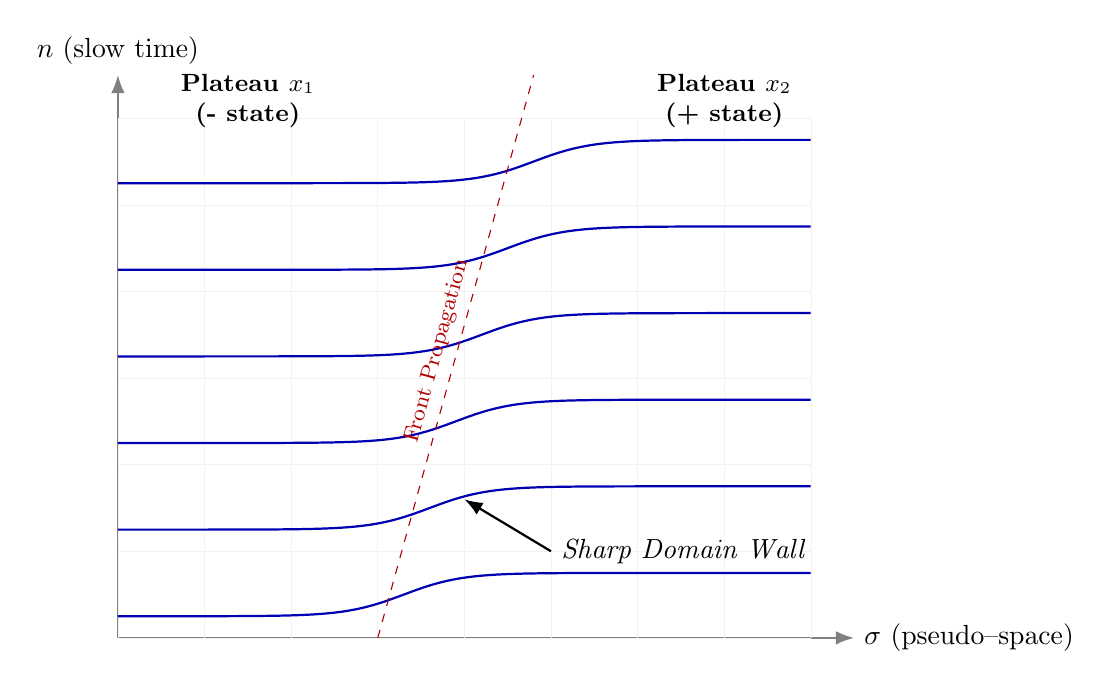
\begin{tikzpicture}[>=Latex, scale=1.1]
                % Axis
                \draw[->, thick, gray] (0,0) -- (8.5,0) node[right, black] {$\sigma$ (pseudo--space)};
                \draw[->, thick, gray] (0,0) -- (0,6.5) node[above, black] {$n$ (slow time)};

                % Grid lines (subtle)
                \draw[step=1cm, gray!10, very thin] (0,0) grid (8,6);

                % Plotting the Fronts using Sigmoid functions
                % Reduced steepness to 1.5 to prevent "Dimension too large" error
                \foreach \y [count=\i] in {0.5, 1.5, ..., 5.5} {
                    \pgfmathsetmacro{\drift}{0.3 * \i}
                    \draw[thick, blue!70!black, domain=0:8, samples=100]
                    plot (\x, {\y + 0.25*tanh(1.5*(\x - 3 - \drift))});
                }

                % Annotations
                \draw[dashed, red!70!black] (3,0) -- (4.8,6.5) node[midway, sloped, above, font=\footnotesize] {Front Propagation};

                \node[font=\bfseries\small, align=center] at (1.5, 6.2) {Plateau $x_1$\\(- state)};
                \node[font=\bfseries\small, align=center] at (7.0, 6.2) {Plateau $x_2$\\ (+ state)};

                % Arrow pointing to a front
                \draw[<-, thick] (4, 1.6) -- (5, 1.0) node[right, font=\itshape] {Sharp Domain Wall};

            \end{tikzpicture}
            \caption{\textbf{Schematic space--time view.} Illustration of the pseudo-space coordinate $\sigma$ versus slow-time index $n$ in the long-delay interpretation. The diagram depicts two plateau-like levels separated by sharp transition layers (fronts), with a small drift per round-trip. In the long-delay regime, such plateau configurations \emph{can} be interpreted as discrete circulation patterns selected by modulational instability.}
            \label{fig:spacetime}
        \end{figure}

        The system exhibits \textbf{multistability}: distinct numbers of plateaus can coexist for the same parameter values, effectively acting as different circulation mode numbers.

    \section*{Numerical Note (Reproducibility)}
        Figure~\ref{fig:spacetime} is a schematic space--time rendering intended to visualize plateau separation and front drift. For reproducible numerical results, Eq.~\eqref{eq:model} can be integrated using a method-of-steps scheme with an explicit Runge--Kutta integrator, specifying (i) step size $\Delta t$, (ii) history function on $[-\tau,0]$, (iii) total integration time in units of $\tau$, and (iv) the parameter ranges $(\mu,\tau/\epsilon)$. We recommend reporting these items explicitly alongside any numerical figure.

    \section*{Global Bifurcations}

        These square--wave families organize into \textit{collapsed snaking} structures. The global topology of solutions is governed by Bykov $T$--points, which act as organizing centers for the creation and destruction of coexisting modes~\cite{stohr2023,bykov1993}.

    \section*{Topological Protection of Circulating Modes}

        The circulating fields of ring systems define Hamiltonian trajectories on a toroidal phase space. As shown by Boozer~\cite{boozer2025}, such Hamiltonian flows generically organize into invariant tori, which act as transport barriers for field lines. Under perturbations, these invariant tori break into \textit{cantori}---fractal remnants that remain extremely effective at suppressing transport---while \textit{turnstiles} provide discrete topological channels for flux transfer between regions.

        These structures suggest that circulating modes in toroidal systems may enjoy partial transport barriers in phase space, in addition to being dynamically selected by delay--induced modulational instability.
        Each plateau configuration identified in Fig.~\ref{fig:spacetime} corresponds to a family of field lines trapped between cantori, with transitions between modes mediated by turnstile dynamics. This offers a possible explanation for the observed robustness of discrete circulating states and their slow decay through rare, topologically constrained transport events.

        Thus, delay--induced pattern formation determines \emph{which} modes appear, while toroidal Hamiltonian topology determines which modes \emph{persist}.

    \section*{Circulating Field Interpretation}

        Any nonlinear loop with finite propagation time—whether optical cavities, electronic delay lines, or electromagnetic resonators—belongs to this universality class.

        In circulation--based field models, the delay $\tau$ corresponds strictly to the loop transit time. Consequently, mode discreteness can arise from classical modulational instability in circulating loops, without introducing ad-hoc quantization rules in the model.


    \section*{Conclusion}
        In the long-delay regime, delayed-feedback dynamics admit a useful spatio--temporal viewpoint in which the delay interval plays the role of a pseudo-spatial domain \cite{giacomelli1996,yanchuk2017}. We argued that, for circulating nonlinear loops, delay-induced modulational instability can select plateau-like configurations that provide a classical route to mode discreteness. We separated this \emph{selection} mechanism from the distinct question of \emph{persistence}, for which transport-barrier concepts (cantori/turnstiles) offer a cautious analogy rather than a derived equivalence \cite{mackay1984,meiss1992,boozer2025}. The framework is intended as a mainstream dynamical-systems interpretation; any SST relevance is motivational and does not rely on nonstandard physical postulates.


    \section*{Discussion}
        \textbf{Delay selection vs.\ persistence.}
        Within the present viewpoint, delay-induced modulational instability can help explain \emph{selection} of plateau configurations in the long-delay regime \cite{giacomelli1996,yanchuk2017}. A separate question is why certain circulating states persist over long times in realistic ring implementations (e.g.\ optical or electronic loops) despite perturbations and weak noise \cite{soriano2013}. One plausible interpretation is that persistence reflects the presence of slow transport channels between coexisting attractors, rather than an absolute barrier.

        \textbf{Analogy to transport barriers in Hamiltonian dynamics.}
        In Hamiltonian transport theory, invariant tori act as barriers that, under perturbation, can break into cantori---partial barriers that still strongly suppress transport---with turnstiles mediating rare flux exchange between regions \cite{mackay1984,meiss1992}. Boozer discusses closely related structures for magnetic field-line dynamics in toroidal plasmas \cite{boozer2025}. While our delay model is not itself a toroidal magnetic field-line map, the \emph{conceptual} analogy suggests a language for ``rare transitions'' between long-lived circulating states: plateau configurations may be metastable and transitions may proceed through narrow dynamical channels rather than by direct smooth deformation.

        \textbf{Relation to Swirl--String Theory (SST) perspective (non-committal).}
        SST treats loop-like propagation and circulation times as structurally important in ring-like excitations. The present delay-based mechanism offers a conservative, classical template for how discrete-looking mode sets can emerge from deterministic pattern selection in a loop, without asserting any direct identification with microscopic quantum postulates. In this manuscript we use the SST connection only as a motivation for further modeling work, not as a claim of equivalence.



    \section*{Outlook}
        Three immediate extensions would strengthen the thesis quantitatively: (i) a bifurcation diagram (e.g.\ numerically continued branches exhibiting multistability and snaking structure), (ii) at least one data-driven figure from Eq.~\eqref{eq:model} demonstrating plateau count as a function of $(\mu,\tau/\epsilon)$, and (iii) a system-specific mapping from a physical ring implementation to effective delay parameters, enabling falsifiable predictions in an optical or electronic loop. From the SST side, a next step would be to identify which circulation times and feedback-like couplings in candidate SST effective models admit an analogous long-delay reduction, and which do not.


%==============================================================================
%   APPENDIX & BIBLIOGRAPHY
%==============================================================================
    \bigskip
    \appendix
    \section*{Appendix A: Sketch of CGLE Reduction}

        Near the Hopf bifurcation threshold ($\mu \approx 1$), the solution can be decomposed as:
        \[
            x(t) = A(\zeta,\theta)\mathrm{e}^{\mathrm{i}\omega t} + \text{complex conjugate}
        \]
        where $\zeta = t/\tau$ is the pseudo-space and $\theta = \epsilon t$ is the slow time. A standard multiple--scale expansion reduces the dynamics to the Complex Ginzburg--Landau Equation (CGLE)~\cite{giacomelli1996}:
        \begin{equation}
            \partial_\theta A = \mu A + (1+\mathrm{i}\alpha)\partial_\zeta^2 A - (1+\mathrm{i}\beta)|A|^2 A.
        \end{equation}
        This equation governs the envelope stability and predicts the onset of domain formation.

        \bigskip
        \begin{thebibliography}{99}
            \setlength{\itemsep}{2pt} % Slightly more space between items

            \bibitem{giacomelli1996}
            Giacomelli, G., and Politi, A. (1996).
            Relationship between delayed and spatially extended dynamical systems.
            \textit{Phys. Rev. Lett.} \textbf{76}, 2686--2689.
            \href{https://doi.org/10.1103/PhysRevLett.76.2686}{doi:10.1103/PhysRevLett.76.2686}

            \bibitem{yanchuk2017}
            Yanchuk, S., and Giacomelli, G. (2017).
            Spatio--temporal phenomena in complex systems with time delays.
            \textit{J. Phys. A: Math. Theor.} \textbf{50}, 103001.
            \href{https://doi.org/10.1088/1751-8121/50/10/103001}{doi:10.1088/1751-8121/50/10/103001}


            \bibitem{stohr2023}
            Stöhr, M. et al. (2023). Square waves and Bykov T--points in a delay algebraic model. \textit{Chaos}, 33, 113105. \href{https://doi.org/10.1063/5.0156262}{doi:10.1063/5.0156262}

            \bibitem{bykov1993}
            Bykov, V. V. (1993). The bifurcations of separatrix connections and chaos. \textit{Physica D}, 62, 290. \href{https://doi.org/10.1016/0167-2789(93)90218-2}{doi:10.1016/0167-2789(93)90218-2}

            \bibitem{boozer2025}
            Boozer, A. H. (2025).
            Magnetic field line chaos, cantori, and turnstiles in toroidal plasmas.
            \textit{arXiv preprint} arXiv:2510.25047.
            \href{https://arxiv.org/abs/2510.25047}{arXiv:2510.25047}


            \bibitem{soriano2013}
            Soriano, M. C., Garc\'ia-Ojalvo, J., Mirasso, C. R., and Fischer, I. (2013).
            Complex photonics: Dynamics and applications of delay-coupled semiconductor lasers.
            \textit{Rev. Mod. Phys.} \textbf{85}, 421--470.
            \href{https://doi.org/10.1103/RevModPhys.85.421}{doi:10.1103/RevModPhys.85.421}

            \bibitem{mackay1984}
            MacKay, R. S., Meiss, J. D., and Percival, I. C. (1984).
            Transport in Hamiltonian systems.
            \textit{Physica D} \textbf{13}, 55--81.
            \href{https://doi.org/10.1016/0167-2789(84)90270-7}{doi:10.1016/0167-2789(84)90270-7}

            \bibitem{meiss1992}
            Meiss, J. D. (1992).
            Symplectic maps, variational principles, and transport.
            \textit{Rev. Mod. Phys.} \textbf{64}, 795--848.
            \href{https://doi.org/10.1103/RevModPhys.64.795}{doi:10.1103/RevModPhys.64.795}

        \end{thebibliography}

\end{document}